% Options for packages loaded elsewhere
\PassOptionsToPackage{unicode}{hyperref}
\PassOptionsToPackage{hyphens}{url}
%
\documentclass[
  ,man,floatsintext]{apa6}
\usepackage{amsmath,amssymb}
\usepackage{iftex}
\ifPDFTeX
  \usepackage[T1]{fontenc}
  \usepackage[utf8]{inputenc}
  \usepackage{textcomp} % provide euro and other symbols
\else % if luatex or xetex
  \usepackage{unicode-math} % this also loads fontspec
  \defaultfontfeatures{Scale=MatchLowercase}
  \defaultfontfeatures[\rmfamily]{Ligatures=TeX,Scale=1}
\fi
\usepackage{lmodern}
\ifPDFTeX\else
  % xetex/luatex font selection
\fi
% Use upquote if available, for straight quotes in verbatim environments
\IfFileExists{upquote.sty}{\usepackage{upquote}}{}
\IfFileExists{microtype.sty}{% use microtype if available
  \usepackage[]{microtype}
  \UseMicrotypeSet[protrusion]{basicmath} % disable protrusion for tt fonts
}{}
\makeatletter
\@ifundefined{KOMAClassName}{% if non-KOMA class
  \IfFileExists{parskip.sty}{%
    \usepackage{parskip}
  }{% else
    \setlength{\parindent}{0pt}
    \setlength{\parskip}{6pt plus 2pt minus 1pt}}
}{% if KOMA class
  \KOMAoptions{parskip=half}}
\makeatother
\usepackage{xcolor}
\usepackage{graphicx}
\makeatletter
\def\maxwidth{\ifdim\Gin@nat@width>\linewidth\linewidth\else\Gin@nat@width\fi}
\def\maxheight{\ifdim\Gin@nat@height>\textheight\textheight\else\Gin@nat@height\fi}
\makeatother
% Scale images if necessary, so that they will not overflow the page
% margins by default, and it is still possible to overwrite the defaults
% using explicit options in \includegraphics[width, height, ...]{}
\setkeys{Gin}{width=\maxwidth,height=\maxheight,keepaspectratio}
% Set default figure placement to htbp
\makeatletter
\def\fps@figure{htbp}
\makeatother
\setlength{\emergencystretch}{3em} % prevent overfull lines
\providecommand{\tightlist}{%
  \setlength{\itemsep}{0pt}\setlength{\parskip}{0pt}}
\setcounter{secnumdepth}{-\maxdimen} % remove section numbering
% Make \paragraph and \subparagraph free-standing
\ifx\paragraph\undefined\else
  \let\oldparagraph\paragraph
  \renewcommand{\paragraph}[1]{\oldparagraph{#1}\mbox{}}
\fi
\ifx\subparagraph\undefined\else
  \let\oldsubparagraph\subparagraph
  \renewcommand{\subparagraph}[1]{\oldsubparagraph{#1}\mbox{}}
\fi
\newlength{\cslhangindent}
\setlength{\cslhangindent}{1.5em}
\newlength{\csllabelwidth}
\setlength{\csllabelwidth}{3em}
\newlength{\cslentryspacingunit} % times entry-spacing
\setlength{\cslentryspacingunit}{\parskip}
\newenvironment{CSLReferences}[2] % #1 hanging-ident, #2 entry spacing
 {% don't indent paragraphs
  \setlength{\parindent}{0pt}
  % turn on hanging indent if param 1 is 1
  \ifodd #1
  \let\oldpar\par
  \def\par{\hangindent=\cslhangindent\oldpar}
  \fi
  % set entry spacing
  \setlength{\parskip}{#2\cslentryspacingunit}
 }%
 {}
\usepackage{calc}
\newcommand{\CSLBlock}[1]{#1\hfill\break}
\newcommand{\CSLLeftMargin}[1]{\parbox[t]{\csllabelwidth}{#1}}
\newcommand{\CSLRightInline}[1]{\parbox[t]{\linewidth - \csllabelwidth}{#1}\break}
\newcommand{\CSLIndent}[1]{\hspace{\cslhangindent}#1}
\ifLuaTeX
\usepackage[bidi=basic]{babel}
\else
\usepackage[bidi=default]{babel}
\fi
\babelprovide[main,import]{english}
% get rid of language-specific shorthands (see #6817):
\let\LanguageShortHands\languageshorthands
\def\languageshorthands#1{}
% Manuscript styling
\usepackage{upgreek}
\captionsetup{font=singlespacing,justification=justified}

% Table formatting
\usepackage{longtable}
\usepackage{lscape}
% \usepackage[counterclockwise]{rotating}   % Landscape page setup for large tables
\usepackage{multirow}		% Table styling
\usepackage{tabularx}		% Control Column width
\usepackage[flushleft]{threeparttable}	% Allows for three part tables with a specified notes section
\usepackage{threeparttablex}            % Lets threeparttable work with longtable

% Create new environments so endfloat can handle them
% \newenvironment{ltable}
%   {\begin{landscape}\centering\begin{threeparttable}}
%   {\end{threeparttable}\end{landscape}}
\newenvironment{lltable}{\begin{landscape}\centering\begin{ThreePartTable}}{\end{ThreePartTable}\end{landscape}}

% Enables adjusting longtable caption width to table width
% Solution found at http://golatex.de/longtable-mit-caption-so-breit-wie-die-tabelle-t15767.html
\makeatletter
\newcommand\LastLTentrywidth{1em}
\newlength\longtablewidth
\setlength{\longtablewidth}{1in}
\newcommand{\getlongtablewidth}{\begingroup \ifcsname LT@\roman{LT@tables}\endcsname \global\longtablewidth=0pt \renewcommand{\LT@entry}[2]{\global\advance\longtablewidth by ##2\relax\gdef\LastLTentrywidth{##2}}\@nameuse{LT@\roman{LT@tables}} \fi \endgroup}

% \setlength{\parindent}{0.5in}
% \setlength{\parskip}{0pt plus 0pt minus 0pt}

% Overwrite redefinition of paragraph and subparagraph by the default LaTeX template
% See https://github.com/crsh/papaja/issues/292
\makeatletter
\renewcommand{\paragraph}{\@startsection{paragraph}{4}{\parindent}%
  {0\baselineskip \@plus 0.2ex \@minus 0.2ex}%
  {-1em}%
  {\normalfont\normalsize\bfseries\itshape\typesectitle}}

\renewcommand{\subparagraph}[1]{\@startsection{subparagraph}{5}{1em}%
  {0\baselineskip \@plus 0.2ex \@minus 0.2ex}%
  {-\z@\relax}%
  {\normalfont\normalsize\itshape\hspace{\parindent}{#1}\textit{\addperi}}{\relax}}
\makeatother

% \usepackage{etoolbox}
\makeatletter
\patchcmd{\HyOrg@maketitle}
  {\section{\normalfont\normalsize\abstractname}}
  {\section*{\normalfont\normalsize\abstractname}}
  {}{\typeout{Failed to patch abstract.}}
\patchcmd{\HyOrg@maketitle}
  {\section{\protect\normalfont{\@title}}}
  {\section*{\protect\normalfont{\@title}}}
  {}{\typeout{Failed to patch title.}}
\makeatother

\usepackage{xpatch}
\makeatletter
\xapptocmd\appendix
  {\xapptocmd\section
    {\addcontentsline{toc}{section}{\appendixname\ifoneappendix\else~\theappendix\fi\\: #1}}
    {}{\InnerPatchFailed}%
  }
{}{\PatchFailed}
\keywords{bilingual infants, cognates, translation equivalents, phonological similarity, expressive vocabulary development}
\usepackage{lineno}

\linenumbers
\usepackage{csquotes}
\usepackage{amsmath}
\usepackage[labelformat=empty]{caption}
\usepackage{caption}
\usepackage[extra]{tipa}
\renewcommand{\topfraction}{1}
\renewcommand{\bottomfraction}{1}
\renewcommand{\textfraction}{.1}
\renewcommand{\floatpagefraction}{1}
\setcounter{topnumber}{9}
\setcounter{bottomnumber}{9}
\setcounter{totalnumber}{20}
\setcounter{dbltopnumber}{9}
\ifLuaTeX
  \usepackage{selnolig}  % disable illegal ligatures
\fi
\IfFileExists{bookmark.sty}{\usepackage{bookmark}}{\usepackage{hyperref}}
\IfFileExists{xurl.sty}{\usepackage{xurl}}{} % add URL line breaks if available
\urlstyle{same}
\hypersetup{
  pdftitle={Cognates are advantaged over non-cognates in early bilingual expressive vocabulary development},
  pdfauthor={Lori Mitchell1, Rachel Ka-Ying Tsui1, \& Krista Byers-Heinlein1},
  pdflang={en-EN},
  pdfkeywords={bilingual infants, cognates, translation equivalents, phonological similarity, expressive vocabulary development},
  hidelinks,
  pdfcreator={LaTeX via pandoc}}

\title{Cognates are advantaged over non-cognates in early bilingual expressive vocabulary development}
\author{Lori Mitchell\textsuperscript{1}, Rachel Ka-Ying Tsui\textsuperscript{1}, \& Krista Byers-Heinlein\textsuperscript{1}}
\date{}


\shorttitle{Cognate advantage in bilingual infants}

\authornote{

Correspondence concerning this article should be addressed to Rachel Ka-Ying Tsui, Department of Psychology, 7141 Sherbrooke St.~West, Montreal, QC, Canada, H2T1V2. Rachel Ka-Ying Tsui is now at Language Development Subgroup of Laboratory for Molecular Mechanism of Brain Development, RIKEN Center for Brain Science, 2-1 Hirosawa, Wako-shi, Saitama, Japan, 351-0198. E-mail: \href{mailto:rachelkytsui@gmail.com}{\nolinkurl{rachelkytsui@gmail.com}}

}

\affiliation{\vspace{0.5cm}\textsuperscript{1} Concordia University}

\abstract{%
Bilinguals need to learn two words for most concepts. These words are called translation equivalents, and those that also sound similar (e.g., banana---\emph{banane}) are called cognates. Research has consistently shown that children and adults process and name cognates more easily than non-cognates. The present study explored if there is such an advantage for cognate production in bilinguals' early vocabulary development. Using longitudinal expressive vocabulary data collected from 47 English--French bilinguals starting at 16--20 months up to 27 months (a total of 219 monthly administrations in both English and French), results showed that overall children produced a greater proportion of cognates than non-cognates, and the interval between producing a word and its translation equivalent was about 10--15 days shorter for cognates than for non-cognates. The findings suggest that cognate learning is facilitated in early bilingual vocabulary development. Just as phonological overlap supports monolinguals in learning phonologically similar words in only one language, phonological overlap also supports bilinguals in learning phonologically similar words across their two languages.
}



\begin{document}
\maketitle

\captionsetup[table]{labelformat=empty}

Infants understand some words during the first year of life, and begin to produce words around their first birthday (Fenson et al., 2007). To do so, infants must represent both the phonological and semantic aspects of a word, and associate the two. Intriguingly, the network of words that children already know appears to shape the words that they will learn: monolingual infants are more likely to learn words that are phonologically (Luce \& Pisoni, 1998; Coady \& Aslin, 2003) and semantically (Coady \& Aslin, 2003) similar to those they already know. Bilingual infants provide a unique perspective into understanding children's developing lexical networks, as they must acquire translation equivalents, which are cross-language synonyms with complete or nearly complete semantic overlap (e.g., ``apple'' in English and \emph{``pomme''} in French; De Houwer et al., 2006; Legacy et al., 2017; Pearson et al., 1995; see White et al.~(2017) for a discussion of convergence in bilinguals' semantic representations). For infants acquiring typologically or historically related languages, some of these translation equivalents will be cognates, which are also phonologically similar (e.g., ``banana'' \textipa{/b@n\ae{}n@/} in English and \emph{``banane''} \textipa{/b\textscripta{}n\textscripta{}n/} in French). This current study aimed to understand the impact of cognate status on the acquisition of words in young bilinguals by examining whether bilingual infants produce cognates more readily than non-cognates in early language development.

\hypertarget{translation-equivalents}{%
\subsection{Translation Equivalents}\label{translation-equivalents}}

Translation equivalents are an important part of early language development for bilingual children. While early researchers claimed that bilinguals avoid learning translation equivalents (Volterra \& Taeschner, 1978), recent work shows that bilingual infants acquire translation equivalents from an early age (Legacy et al., 2017; Pearson et al., 1995). Bilingual infants begin to produce translation equivalents by 16 months, and produce more translation equivalents with age as their vocabularies grow (Legacy et al., 2017). The strong semantic overlap of a word in one language seems to facilitate the acquisition of its translation equivalent in the other language, at least at younger ages when bilingual infants have smaller vocabularies (Bilson et al., 2015; Tsui et al., 2022). By the age of 27 months, bilingual toddlers recognize a target word more accurately when preceded by its translation equivalent (Floccia et al., 2020).

For bilingual infants, some translation equivalents sound very similar. Specifically, cognates are a type of translation equivalents that have significant phonological overlap, typically due to a shared etymology\footnote{Cognates can also overlap in their orthography, but we do not address orthography in this paper as our participants were too young to read.}. Cognates range in their degree of phonological similarity: For example, English ``banana'' \textipa{/b@n\ae{}n@/} and French \emph{``banane''} \textipa{/b\textscripta{}n\textscripta{}n/} are highly phonetically similar, while English ``pants'' \textipa{/p\ae{}nts/} and French \emph{``pantalon''} \textipa{/p\~A tAl\~O/} are more different including a different number of syllables. Some typologically close languages even have form-identical cognates, such as the word \emph{``sí''} \textipa{/si/} which means ``yes'' in both Spanish and Catalan.

Cognates appear to have a special status in bilingual language processing and production. Previous research has reported a cognate facilitation effect where bilinguals are better and quicker at identifying and naming cognates than non-cognates when performing vocabulary tasks (e.g., Costa et al., 2000; Kelley \& Kohnert, 2012; Sheng et al., 2016). This type of advantage for cognates has been reported in bilingual adults (e.g., Costa et al., 2000) as well as in school-aged children (e.g., Kelley \& Kohnert, 2012; Sheng et al., 2016). For example, Kelley and Kohnert (2012) provide evidence for the cognate facilitation effect in Spanish-speaking English learners between the ages of 8 and 13 years old, where children identified and named more cognates than non-cognates in receptive and expressive vocabulary tasks. A similar cognate advantage has been found for picture naming and translation tasks for English--Spanish and English--German 4- to 8-year-old children where bilingual children were more accurate in naming cognates and faster at translating cognates than non-cognates (Schelletter, 2002; Sheng et al., 2016). Therefore, cognates seem to be advantaged in school-aged bilingual children's language processing and production.

\hypertarget{effects-of-phonological-similarity-on-early-word-learning}{%
\subsection{Effects of Phonological Similarity on Early Word Learning}\label{effects-of-phonological-similarity-on-early-word-learning}}

The advantage for cognates could be attributed to the phonological overlap between words, which may make them easier to learn. Existing literature on monolinguals has reported that children are more likely to produce words that sound similar to other words in their lexicons (e.g., ``at'' and ``cat,'' ``hat'' and ``cat''), especially at younger ages (e.g., Jones \& Brandt, 2019). For instance, looking at 300 British English-speaking children aged 12 to 25 months, Jones and Brandt (2019) found that the strength of phonological similarity between words was an important predictor for word production (but not comprehension), whereby young children tended to produce words that follow similar phonological patterns. Similarly, using archival expressive vocabulary data from 1,800 16- to 30-month-old American infants, it was shown that infants produced more nouns with many phonological neighbours than those with few phonological neighbours (Storkel, 2009). It is possible that the high degree of phonological similarity aids word acquisition through sounds already established in the lexicons. For example, Demke et al.~(2002) found that hearing real-word phonological neighbours facilitated the learning of new pseudowords. Another possibility is that the words that share a high degree of phonological similarity in the language input are learned first by infants, as supported by a recent study looking at the developing lexicons of young infants across 10 languages (Fourtassi et al., 2020). Overall, learning a new word with close phonological neighbours seems to help learners maintain the new word in memory, making similar-sounding words easier to acquire and produce (e.g., Coady \& Aslin, 2003; Demke et al., 2002; Jones \& Brandt, 2019).

Extending this notion to bilingual infants, some evidence suggests that phonological similarity facilitates vocabulary learning across languages as well. For example, Gampe et al.~(2021) examined parent-reported vocabulary size of 18- to 36-month-old children learning Swiss German and another language. Children learning languages that were more phonologically similar to Swiss German (e.g., standard German, Dutch, English) produced more words than children learning languages that were more phonologically dissimilar (e.g., Turkish, French). Moreover, children learning more similar languages learned more cognate translation equivalents, while the number of non-cognate translation equivalents was similar across groups. These results are consistent with other studies reporting that language distance affects early bilingual language acquisition (e.g., Blom et al., 2019; Gampe et al., 2021; Havy et al., 2016; Sheng et al., 2016).

However, not all studies have reported a generalized advantage for cognates in vocabulary learning. In a study of younger children, Bosch and Ramon-Casas (2014) used parent reports to examine word production in 18-month-olds learning Spanish and Catalan, two strongly related languages that share many form-identical (e.g, ``yes'' is \emph{``sí''} \textipa{/si/} in both Spanish and Catalan) and form-similar (e.g., ``hand'' is \emph{``mano''} \textipa{/mAno/} in Spanish and \emph{``mà''} \textipa{/mA/} in Catalan) cognates. Results indicated that 28\% of the words produced by the bilingual infants were form-identical cognates, while less than 2\% of words were form-similar cognates or non-cognate translation equivalents (Bosch \& Ramon-Casas, 2014). One explanation for this finding is that for form-identical cognates, infants only need to learn a single form for a particular concept, which they can then transfer across their languages. Based on these results, bilingual infants may not benefit from cognates' phonological overlap unless that overlap is perfect. Indeed, there is some evidence that Spanish--Catalan infants are somewhat insensitive to phonological distinctions in form-similar cognates (Ramon-Casas et al., 2009; Ramon-Casas \& Bosch, 2010), perhaps even representing them as form-identical. Another interpretation of this result is that the effect of cognates on bilingual vocabulary learning changes across development, which could explain the discrepant results of the 18-month-old sample studied by Bosch \& Ramon-Casas (2014), and the 18- to 36-month-old sample studied by Gampe et al.~(2021). Specifically, it is possible that an advantage for cognates is detectable first for form-identical cognates when they are present in the languages (as in Bosch \& Ramon-Casas, 2014), and then later for form-similar cognates as children grow older and learn more words overall (as in Gampe et al., 2021). In other words, cognate status and age might interact.

\hypertarget{current-study}{%
\subsection{Current study}\label{current-study}}

To better understand the impact of phonological overlap on bilingual infants' vocabulary learning, we examined the production of cognate and non-cognate translation equivalents in French--English bilingual infants. English and French share many form-similar cognates due to historical language contact (Choi, 2019), although only a few form-identical cognates. Despite the presence of cognates, note that these two languages belong to different language families: English is a Germanic language and French is a Romance language. Previous work looked at learners of closely related languages with many form-identical cognates (Spanish and Catalan; Ramon-Casas \& Bosch, 2010), or else a heterogeneous group of bilinguals learning many different language pairs (Gampe et al., 2021). Thus, our study provided an important test of the generalizability of these results in a new and homogeneous population of young bilinguals.

We collected monthly vocabulary data on French--English bilingual infants' word production starting when children were between the ages of 16--20 months and ending when were up to 27 months of age using the MacArthur-Bates Web-Communicative Developmental Inventory: Words and Sentences form in American English (Fenson et al., 2007) and Québec French (Trudeau et al., 1999). Uniquely, our dataset was longitudinal, allowing us to investigate potential developmental effects. We focused our analysis on translation equivalent pairs and then classified the pairs according to cognate status (cognate or non-cognate words). We counted children's production of both translation equivalent pairs (e.g., whether they produced both ``apple'' \textipa{/\ae{}p@l/} and \emph{``pomme''} \textipa{/p\textopeno{}m/}, or both ``banana'' \textipa{/b@n\ae{}n@/} and \emph{``banane''} \textipa{/b\textscripta{}n\textscripta{}n/}), as well as individual words independent of whether children produced its translation equivalent. Since it is not possible to randomly assign our main variable of interest (cognate status), we analyzed both a complete list of cognate and non-cognate words, as well as a carefully selected subset of these cognate and non-cognate words which were matched on age of acquisition and on word category (e.g., words about food) where possible.

We hypothesized that French--English bilinguals would more readily produce cognates than non-cognates. Thus, we predicted that French--English bilingual infants would produce proportionally more translation equivalent words and pairs that were cognates than non-cognates. We likewise anticipated an interaction between cognate status and age, with a stronger effect of cognate status at older ages as the infants' vocabulary size (and the number of translation equivalent words and pairs produced) grew. We also explored whether the interval between producing a word and its translation equivalent would be shorter for cognates than for non-cognates.

\hypertarget{method}{%
\section{Method}\label{method}}

The present research was approved by the Human Research Ethics Committee at Concordia University {[}certification \#10000439{]}. Participation was on a voluntary basis and the families were free to withdraw at any time. The study design and data analysis plan were pre-registered at \url{https://osf.io/6fk8r/}. Any deviations from the pre-registration are listed and justified in the supplemental materials, available at \url{https://osf.io/rh7av/}.

\hypertarget{participants}{%
\subsection{Participants}\label{participants}}

The current study comprised data from 50 French--English bilingual infants (26 females) which were collected from August 2020 to May 2021 during part of a larger ongoing longitudinal study. Participating infants were aged between 16 and 20 months at the onset of participation (mean starting age = 17.98 months, SD = 1.15, range = 16.20 -- 20.40), and were aged between 16 to 27 months at their final time of participation (M = 21.96 months, SD = 3.20, range = 16.30 -- 27.14). Participants were recruited from Québec, Canada through government birth lists, social media, and participating families' referrals. Inclusion criteria were the following: full-term pregnancy (i.e., at least 37 weeks of gestation), normal birth weight (\textgreater{} 2500 grams), and no reported developmental delays or any hearing or vision problems. Bilingual infants were defined as those exposed to each of English and French for at least 10\% and at most 90\% of the time over the course of their lives since birth, with less than 10\% of exposure to a third language\footnote{We have also run the analyses using a stricter 25\%-75\% inclusion criterion. The results are consistent with the main analysis, and are reported in the supplemental materials.}. To capture a wider range of bilingual experience, the language exposure range in this study was wider than some studies (e.g., Morin-Lessard \& Byers-Heinlein, 2019; Sebastián-Gallés \& Bosch, 2009) but similar to the range used in others (e.g., Hoff \& Ribot, 2017; Place \& Hoff, 2011).

In total, parents completed 230 English CDI administrations and 226 French CDI administrations, which constitutes a large dataset particularly in the context of research with bilingual infants (Rocha-Hidalgo \& Barr, 2022). We retained only cases where both the English and French were completed at the same time point to be able to determine infants' translation equivalent knowledge. This left us with 219 completed administrations from 47 infants. Six infants contributed data at only one time point, and 41 infants contributed data at more than one time point, with participants contributing an average of 4.70 measurements for each language (SD = 2.51, range = 1 -- 10). On average across the 219 administrations, participating infants were exposed to English 48.8\% of the time (SD = 17.3, range = 11 -- 84), to French 50.6\% of the time (SD = 17.7, range = 16 -- 88), and to a third language 0.6\% of the time (SD = 1.5, range = 0 -- 5). Of the 47 bilingual infants, 26 were English-dominant (M = 60.1\% English exposure, SD = 10, range = 49 -- 84), 20 were French-dominant (M = 66.4\% French exposure, SD = 12.7, range = 51 -- 88), and 1 reported equal exposure to both English and French. The average maternal education level was 17.32 years (SD = 2.29, range = 12 -- 23), and 89.40\% of the mothers had completed a university degree or higher.

\hypertarget{measures}{%
\subsection{Measures}\label{measures}}

\hypertarget{web-based-macarthur-bates-communicative-development-inventory-words-and-sentences-web-cdi}{%
\subsubsection{Web-based MacArthur-Bates Communicative Development Inventory: Words and Sentences (Web-CDI)}\label{web-based-macarthur-bates-communicative-development-inventory-words-and-sentences-web-cdi}}

The number of words produced in English and French was obtained monthly via the web-based versions of the MacArthur-Bates Web-Communicative Development Inventories: Words and Sentences form (Web-CDI; \url{https://webcdi.stanford.edu/}), using the American English version (Fenson et al., 2007) and the Québec French adaptation (``Mots et Énoncés''; Trudeau et al., 1999). Our study focused on the vocabulary checklist component of the CDIs, with 680 words in the English version and 664 words in the Québec French version. We asked the caregiver most familiar with the infant's vocabulary in each language to complete the respective version, although following the instructions on the Web-CDI they could seek help from others who often speak the corresponding language with the infant. The English forms were completed by mothers (88\%), fathers (7\%), and both parents (5\%), whereas the French forms were completed by mothers (84\%), fathers (11\%), and both parents (5\%). Thus, most of the time, the same caregiver (usually the mother) filled out both forms. Generally, whichever caregiver completed forms in a particular language did so throughout the study, with the exception of 2 participants (4.3\%) whose English forms were filled out by different caregivers for some administrations, and 3 participants (6.4\%) whose French forms were filled out by different caregivers for some administrations. Infants' demographic information including age and sex was also collected at the start of the Web-CDI.

\hypertarget{language-exposure-questionnaire-leq-using-the-multilingual-approach-to-parent-language-estimates-maple}{%
\subsubsection{Language Exposure Questionnaire (LEQ) using the Multilingual Approach to Parent Language Estimates (MAPLE)}\label{language-exposure-questionnaire-leq-using-the-multilingual-approach-to-parent-language-estimates-maple}}

The infant's language exposure and background was measured with an adaptation of the Language Exposure Questionnaire (LEQ; Bosch \& Sebastián-Gallés, 2001), using the Multilingual Approach to Parent Language Estimates (MAPLE; Byers-Heinlein et al., 2020). During a 15- to 20-minute structured interview, the primary caregiver(s) were asked questions about the infant's language exposure from birth until their current age. This provided a global estimate of the percentage of exposure that the infant had to each of their languages across all contexts.

\hypertarget{procedure}{%
\subsection{Procedure}\label{procedure}}

Data collection for this study began in August 2020 and ended in May 2021, although the start date of participation varied across participants. On the first day of each month, links to the English and French Web-CDI forms were sent to the caregivers by email. On the forms, the words that were checked off in previous months were automatically filled in the following months; thus, caregivers only needed to check off the new words that their child produced each month. This was intended to reduce the burden on participants, and increase the response rate. Parents were instructed to consider the word produced even if the child's production was not adult-like (e.g., the child produced ``raff'' instead of ``giraffe''). We asked that the Web-CDI forms be completed during the first week of each month. A reminder was sent on the 8th of the month, and an extra week was given for caregivers who had not yet completed the forms. If caregivers still did not complete the form, they were asked to resume their participation the following month. Once the forms were completed, caregivers received a brief report about their child's vocabulary knowledge at that time point, including the total number of words that their child produced as well as the breakdown of the categories (such as animals, food, furniture, etc.) for which their child produced words.

At the first data collection time point, caregivers also completed the LEQ questionnaire with a trained research assistant over the online video chat application Zoom. This was repeated every five months to track any potential changes in the infant's language exposure. This was particularly important as data collection overlapped with the COVID-19 pandemic, thus it was important to closely track language exposure changes due to lockdowns, return to daycare, etc.

\hypertarget{identification-of-translation-equivalents-and-cognates}{%
\subsection{Identification of Translation Equivalents and Cognates}\label{identification-of-translation-equivalents-and-cognates}}

A list of translation equivalents on the English and French forms of the CDI was determined in the same manner as Byers-Heinlein et al.~(2023), and was created by three proficient English--French bilingual adults who carefully examined the English and French versions of the CDIs\footnote{In cases of disagreement, the three raters discussed the likely uses of the word in question by children (rather than potential adult uses of the same word) and then reached a decision together.}; a total of 611 translation equivalent pairs were identified (the full list is available at \url{https://osf.io/7fz6c/}; methodological details are reported in Tsui et al., 2022). Next, the bilingual research assistants judged how similar the translation equivalent pairs sounded; they identified 138 of the possible 611 translation equivalent pairs as cognates, with the remaining 473 words as non-cognates. Phonological similarity of the identified cognates were further confirmed by a separate group of bilingual undergraduate students who listened to recordings of the translation equivalent pairs and were asked to rate how similar those words sounded. This method was preferred to other methods that focus on orthography (overlap in spelling), since infants acquire language through spoken words as opposed to reading.

From the list of 611 translation equivalents, we further excluded any translation equivalent pairs that had complex relationships rather than one-to-one mappings. For example, ``noodle'' forms a translation equivalent pair with either the French word \emph{``nouilles''} or \emph{``pâtes''}, where both French words are listed together as one item on the French CDI form. These pairs were removed because we could not know which form (e.g., \emph{``nouilles''} or \emph{``pâtes''}) the infant produced, and we were not able to classify these pairs as either cognates or non-cognates.

Following this procedure identified a complete list of 537 translation equivalents (131 cognates\footnote{Among these 131 cognates on the complete list, we could identify 11 cognates that were potentially form-identical: ``choo choo'', ``grr'', ``meow'', ``vroom'', ``woof'', ``Cheerios'', ``Coke'', ``pizza'', ``muffin'', ``toast'', and ``jeans'' (only the last three were on the matched list). Note that each of these words was either a sound effect, a brand name, or a conventionalized borrowing. Even for these words, adult speakers often pronounce them slightly differently in French and English such that words align with each language's phonology, for example differences in the exact realization of particular phonemes, and stress pattern differences in bisyllabic words ``muffin'' and ``pizza''.} and 406 non-cognates), which were compared in a first set of analyses. However, note that the cognates and non-cognates in this list could vary systematically on correlated factors including variations in parts of speech and differences in age of acquisition of certain words between languages. Within the full list of translation equivalents, we thus identified a matched subset of cognates and non-cognates that were compared in a second set of analyses.

Our procedure for identifying the matched list was pre-registered, and designed to minimize potential experimenter biases. The matched list was first restricted to nouns as infants show a noun bias in language acquisition (Caselli et al., 1995), and doing so matched the cognates and non-cognates for part of speech. Next, the remaining 272 translation equivalents (cognates = 90, non-cognates = 182) were matched on age of acquisition and word category where possible (e.g., food, furniture, etc.). However, data on age of acquisition, which was obtained from the wordbankr package (Version 0.3.1; Frank et al., 2017), was not available for 41 translation equivalents which were therefore removed, leaving 231 possible items (cognates = 81, non-cognates = 150). Using the optmatch package (Version 0.9.14; Hansen \& Klopfer, 2006) in the R statistical language (R Core Team, 2019), each cognate item was matched to a non-cognate item according to the typical age of acquisition in both English and French for monolinguals obtained from the wordbankr package (Version 0.3.1; Braginsky, 2018) with the closest match possible on word category. There were 52 pairs that matched exactly based on these criteria. For example, the cognate pair ``chair''--\emph{``chaise''} and the non-cognate pair ``bed''--\emph{``lit''} matched because they are typically acquired at age 21 months by monolinguals in English and French and are both in the furniture category (Frank et al., 2017). The remaining 29 pairs were matched on age of acquisition as well, allowing a possible one-month deviation in either English, French or both. For example, the cognate pair ``mittens''--\emph{``mitaine''} and the non-cognate pair ``slipper''--\emph{``pantoufle''} matched since the English words are acquired at 28 and 27 months respectively (one-month deviation), both French words are acquired at 22 months of age (Frank et al., 2017), and both are clothing. Thus, the final items (81 cognates\footnote{Among these 81 cognates on the matched list, there are 3 form-identical cognates and 78 form-similar cognates.}, 81 non-cognates) included in the matched list were as similar as possible in all respects except their cognate status.

\hypertarget{analytical-strategy}{%
\subsection{Analytical Strategy}\label{analytical-strategy}}

Pre-registered analyses were run on two different dependent variables to examine whether bilingual infants would produce more cognates than non-cognates over their vocabulary development. The first dependent variable was the proportion of items on the word list that infants produced, where translation equivalents were counted as separate items. For example, the word ``banana'' would be counted as a produced cognate, whether or not its translation equivalent \emph{``banane''} was produced. The second dependent variable was the proportion of translation equivalent pairs infants produced. Here, pairs were counted only if the infant produced both items in a pair. For example, the pair ``banana''--\emph{``banane''} was counted as a produced cognate pair if and only if the child could produce both words in the pair. We additionally conducted an exploratory analysis that examined whether the effect of cognates would impact the interval between learning to produce a first and a second word in a translation equivalent pair.

For each dependent variable, we conducted analyses using (1) the complete list of cognates and non-cognates (537 translation equivalents pairs in total) and then restricted the analysis to (2) a matched list (nouns only and matched on age of acquisition;162 translation equivalent pairs in total). Based on the three dependent variables and the two sets of words, we therefore ran a total of four models for the pre-registered analyses, and two models for the exploratory analyses. Linear or logistic mixed-effects analyses, as appropriate, were performed in the R statistical language (Version 4.0.2; R Core Team, 2019) using the lme4 package (Bates et al., 2015). Mixed-effects models are appropriate for repeated measures data (Cnaan et al., 1997). This type of model also accounts for missing data and does not require each participant to contribute the same number of datapoints. Logistic models were appropriate for the pre-registered analyses as our dependent variable was a proportion, and linear models were appropriate for the exploratory analysis as our dependent variable was continuous. For the pre-registered analysis, regression weights reflected the total number of cognates and non-cognates to account for the different number of words between the cognate and non-cognate lists. The lmerTest package (Kuznetsova et al., 2017) was used to calculate p-values. Goodness-of-fit tests for the mixed-effects models were estimated using the DHARMa package (Hartig, 2022). Analysis scripts and the data set used in the present study are available at {[}\url{https://osf.io/rh7av/}{]}.

\hypertarget{results}{%
\section{Results}\label{results}}

\hypertarget{descriptive-measures-of-number-of-words-produced}{%
\subsection{Descriptive Measures of Number of Words Produced}\label{descriptive-measures-of-number-of-words-produced}}

Out of the complete list (a possible 537 translation equivalent pairs with 537 × 2 = 1074 words), bilingual infants on average produced a total of 157 words (SD = 158), with a range of 0 -- 709 words, which constituted 14.6\% of the words on the complete list. Moreover, bilingual infants produced an average of 39 complete translation equivalent pairs where both the English and French words were produced (SD = 50.61, range = 0 -- 243), which constituted 7.3\% of the translation equivalent pairs on the complete list.

Restricting to the matched list which contained 162 translation equivalent pairs with 162 × 2 = 324 words, bilingual infants produced an average of 51 words (SD = 59.71, range = 0 -- 248), which constituted 15.7\% of the words on the matched list. On average, bilingual infants produced a total of 12 complete translation equivalent pairs (SD = 20.77, range = 0 -- 92), which constituted 7.6\% of translation equivalent pairs on the matched list.

\hypertarget{dependent-variable-1-cognate-words-versus-non-cognate-words}{%
\subsection{Dependent Variable 1: Cognate Words Versus Non-Cognate Words}\label{dependent-variable-1-cognate-words-versus-non-cognate-words}}

In this analysis, the dependent variable was the total proportion of words infants produced on the relevant list. Proportion was used as opposed to raw number of words to provide a more comparable description of production of cognates versus non-cognates, since the number of cognate words and non-cognates words differed especially in the complete list. Our predictor variables were age (in days) and cognate status. Age was continuous and was centered at the mean age of 547.6 days (approximately 18 months) for ease of interpretation. Cognate status was categorical with two levels (cognates versus non-cognates) with non-cognates as the reference level. We ran separate logistic regression models for the complete and matched lists. The initial model specification included a random slope of age and cognate status by participants, which was pruned to a random intercept to achieve model convergence. The final model was:

proportion\_word \textasciitilde{} age * cognate\_status + (1\textbar participant)

\hypertarget{complete-list}{%
\subsubsection{Complete List}\label{complete-list}}

Out of the complete list which contained 262 cognate words (i.e., adding the 131 English cognate words and 131 French cognate words) and 812 non-cognate words (i.e., adding the 406 English non-cognate words and 406 French non-cognate words), bilingual infants produced an average of 54 cognate words (SD = 45.56, range = 0 -- 204) and 103 non-cognate words (SD = 113.09, range = 0 -- 505). The proportion of cognate words produced was 0.21 (SD = 0.17, range = 0 -- 0.78), whereas the proportion of non-cognate words produced was 0.13 (SD = 0.14, range = 0 -- 0.62). A Q-Q plot visualization and goodness-of-fit tests on the model's residuals showed that our model had a good model fit, \emph{D} = 0.06, \(p = .125\). Table 1 shows the coefficient estimates for the model and Figure 1 Panel A visualizes the model. We observed significant main effects of age and cognate status, as well as a significant interaction. Overall, the pattern of results indicated that infants produced a greater proportion of cognates than non-cognates, with a slightly steeper learning curve for non-cognates than for cognates, although non-cognate production did not ``catch up'' to cognate production during the ages we observed.

\hypertarget{matched-list}{%
\subsubsection{Matched List}\label{matched-list}}

Out of the 162 cognate (i.e., adding the 81 English cognate words and 81 French cognate words) and 162 non-cognate words (i.e., adding the 81 English non-cognate words and 81 French non-cognate words) on the matched list, bilingual infants produced an average of 27 cognate words (SD = 31.52, range = 0 -- 135) and 23 non-cognate words (SD = 28.4, range = 0 -- 113). The overall mean proportion of cognate words produced was 0.17 of words (SD = 0.19, range = 0 -- 0.83), whereas the proportion of non-cognate words produced was 0.14 (SD = 0.18, range = 0 -- 0.7). A Q-Q plot visualization as well as goodness-of-fit tests on the model's residuals showed a good model fit, \emph{D} = 0.06, \(p = .095\). Table 1 also shows the coefficient estimates for the matched list model and Figure 1 Panel B visualizes the model. Similar to the patterns reported in the complete list model, there were significant effects of age and cognate status, once again showing that infants produced a greater proportion of cognates than non-cognates on the matched list. However, for the matched list there was no interaction between cognate status and age, indicating that the magnitude of the cognate advantage for this list was stable as infants grew older.

\begin{figure}[H]

{\centering 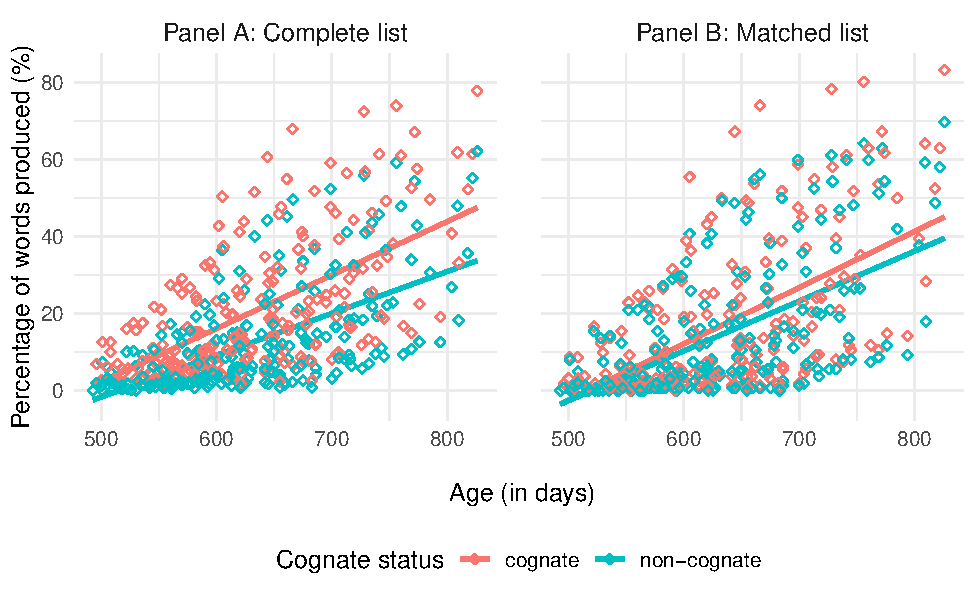
\includegraphics[width=1.2\linewidth]{CogVocab_paper_files/figure-latex/Fig1-1} 

}

\caption{Proportion of words produced by age and cognate status, with Panel A representing the complete list and Panel B representing the matched list. Note that the black dashed line represents the mean age of 547.6 days which serves as the reference level for age in our models.}\label{fig:Fig1}
\end{figure}

\begin{table}[H]

\begin{center}
\begin{threeparttable}

\caption{\label{tab:Table 1}Table 1. Coefficient estimates from the logistic mixed-effects models predicting proportion of words produced.}

\begin{tabular}{lcccccccc}
\toprule
 & \multicolumn{4}{c}{Complete list} & \multicolumn{4}{c}{Matched list} \\
\cmidrule(r){2-5} \cmidrule(r){6-9}
 & Estimate & $SE$ & $z$ & $p$ & Estimate & $SE$ & $z$ & $p$\\
\midrule
Intercept & -2.52 & 0.15 & -16.82 & <.001 & -2.69 & 0.21 & -12.52 & <.001\\
cognate\_status & 0.74 & 0.01 & 49.46 & <.001 & 0.23 & 0.03 & 8.86 & <.001\\
age\_days & 0.01 & 0.00 & 83.17 & <.001 & 0.01 & 0.00 & 45.17 & <.001\\
cognate\_status * age\_days & 0.00 & 0.00 & -5.12 & <.001 & 0.00 & 0.00 & 0.93 & 0.351\\
\bottomrule
\end{tabular}

\end{threeparttable}
\end{center}

\end{table}

\hypertarget{dependent-variable-2-cognate-pairs-versus-non-cognate-pairs}{%
\subsection{Dependent Variable 2: Cognate Pairs Versus Non-Cognate Pairs}\label{dependent-variable-2-cognate-pairs-versus-non-cognate-pairs}}

In this analysis, the proportion of translation equivalent pairs produced was entered as the dependent variable. Age and cognate status were entered as our predictor variables, with non-cognates set as the reference level. Again, we ran separate logistic models for the complete and matched lists. The initial model specification, which included a random effect of age and cognate status by participants, had to be reduced for model convergence; therefore, the final model was:

proportion\_pair \textasciitilde{} age * cognate\_status + (1\textbar participant)

\hypertarget{complete-list-1}{%
\subsubsection{Complete List}\label{complete-list-1}}

Out of the complete list which contained 537 translation equivalent pairs (131 cognates and 406 non-cognates), infants produced an average of 17 cognate pairs (SD = 18.1, range = 0 -- 82) and 22 non-cognate pairs (SD = 32.93, range = 0 -- 167). The proportion of cognate pairs produced was 0.13 (SD = 0.14, range = 0 -- 0.63) whereas the proportion of non-cognate pairs produced was 0.05 (SD = 0.08, range = 0 -- 0.41). A Q-Q plot visualization and goodness-of-fit tests on the model's residuals revealed that our model showed a good model fit, \emph{D} = 0.04, \(p = .398\). Table 2 shows the coefficient estimates for the model and Figure 2 Panel A visualizes the model. There were significant effects of age and cognate status, showing that overall infants produced a greater proportion of cognates than non-cognates. Similar to the pattern reported in the first set of analyses, the interaction between age and cognate status suggested a slightly steeper learning curve for non-cognates than cognates, although an advantage for cognates was still apparent even at 27 months.

\hypertarget{matched-list-1}{%
\subsubsection{Matched List}\label{matched-list-1}}

Out of the 162 translation equivalent pairs, bilingual infants produced an average of 7 cognate pairs (SD = 12.21, range = 0 -- 58) and 5 non-cognate pairs (SD = 8.83, range = 0 -- 42). The proportion of cognate pairs produced was 0.09 (SD = 0.15, range = 0 -- 0.72) and the proportion of non-cognate pairs produced was 0.06 (SD = 0.11, range = 0 -- 0.52). A Q-Q plot visualization and the goodness-of-fit test on the model's residuals (\emph{D} = 0.09, \(p = .002\)) suggested that the logistic model did not fully capture the distribution of the data, but we nevertheless retained the model on theoretical grounds (the dependent variable was proportion) and to facilitate comparison to the previous models. The coefficient estimates for the matched list model is shown in Table 2, and Figure 2 Panel B visualizes the model. Similar to the results for the complete list, the main effects of age and cognate status were statistically significant, showing that infants produced a larger proportion of cognates than non-cognates. However, unlike the results for the complete list, the interaction between age and cognate status was not statistically significant, showing that the magnitude of the cognate difference was reasonably stable across age.

\begin{figure}

{\centering 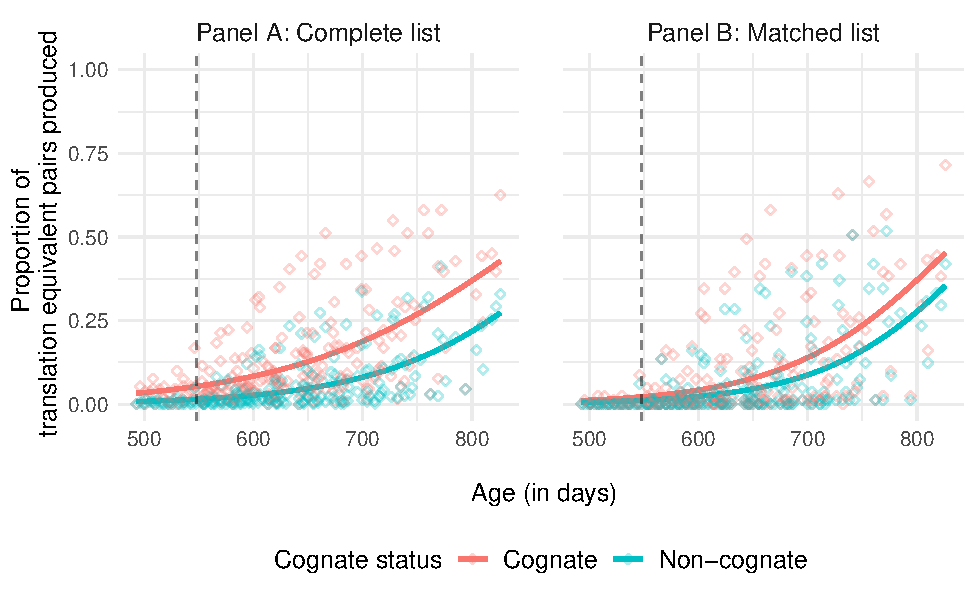
\includegraphics[width=1.2\linewidth]{CogVocab_paper_files/figure-latex/Fig2-1} 

}

\caption{Proportion of translation equivalent pairs produced by age and cognate status, with Panel A representing the complete list and Panel B representing the matched list. Note that the black dashed line represents the mean age of 547.6 days which serves as the reference level for age in our models.}\label{fig:Fig2}
\end{figure}

\begin{table}[tbp]

\begin{center}
\begin{threeparttable}

\caption{\label{tab:Table 2}Table 2. Coefficient estimates from the logistic mixed-effects models predicting proportion of translation equivalent pairs produced.}

\begin{tabular}{lcccccccc}
\toprule
 & \multicolumn{4}{c}{Complete list} & \multicolumn{4}{c}{Matched list} \\
\cmidrule(r){2-5} \cmidrule(r){6-9}
 & Estimate & $SE$ & $z$ & $p$ & Estimate & $SE$ & $z$ & $p$\\
\midrule
Intercept & -3.68 & 0.15 & -24.19 & <.001 & -4.32 & 0.25 & -17.11 & <.001\\
cognate\_status & 1.21 & 0.03 & 41.20 & <.001 & 0.66 & 0.06 & 10.79 & <.001\\
age\_days & 0.01 & 0.00 & 46.44 & <.001 & 0.01 & 0.00 & 25.78 & <.001\\
cognate\_status * age\_days & 0.00 & 0.00 & -6.10 & <.001 & 0.00 & 0.00 & -0.86 & 0.391\\
\bottomrule
\end{tabular}

\end{threeparttable}
\end{center}

\end{table}

\hypertarget{exploratory-analysis-interval-between-producing-translation-equivalents}{%
\subsection{Exploratory Analysis: Interval between Producing Translation Equivalents}\label{exploratory-analysis-interval-between-producing-translation-equivalents}}

In an exploratory analysis, we examined the interval between learning to produce a first word in a translation equivalent pair and learning to produce the second word, as a function of whether the pairs were cognates or non-cognates. Analyses were limited to cases where both words within a translation equivalent pair were eventually produced by an infant within this longitudinal data set. In other words, for each infant we removed translation equivalents in which that infant did not produce any word or only produced one of words during the course of the study. We further removed those translation equivalent pairs where a first word was already produced during the first month of participation, as it may misrepresent the actual month in which the infants first produced that word. Therefore, translation equivalent pairs retained in the following analysis focused on those where an infant learned to produce both words in a pair during the course of their participation.

After such exclusion criteria, it left us with a total of 384 translation equivalent pairs (113 cognate and 271 non-cognate pairs) on the complete list and 137 translation equivalent pairs (73 cognate and 64 non-cognate pairs) on the matched list. While the total number of pairs produced differed across infants, on average each infant produced 16 cognate pairs (\(SD\) = 17.71, range = 1 -- 81) and 29 non-cognate pairs (\(SD\) = 36.86, range = 1 -- 133) on the complete list, and 12 cognate pairs (\(SD\) = 13.73, range = 1 -- 58) and 10 non-cognate pairs (\(SD\) = 10.85, range = 1 -- 34) on the matched list.

For each pair, we calculated the number of days in between when the first word of a pair was produced and when its translation equivalent was produced. For example, if an infant was reported to produce the English word ``dog'' at 548 days (i.e., 18 months) and the French translation equivalent word ``chien'' at 608 days (i.e., 20 months), the interval for this word pair would be 60 days. We then used the interval for each word pair as a dependent variable in a linear mixed-effects model, with cognate status as fixed effects (with non-cognates as the reference level), and participants and word pairs as random intercepts:

interval\_days \textasciitilde{} cognate\_status + (1\textbar participant) + (1\textbar word\_pair)

\begin{figure}

{\centering 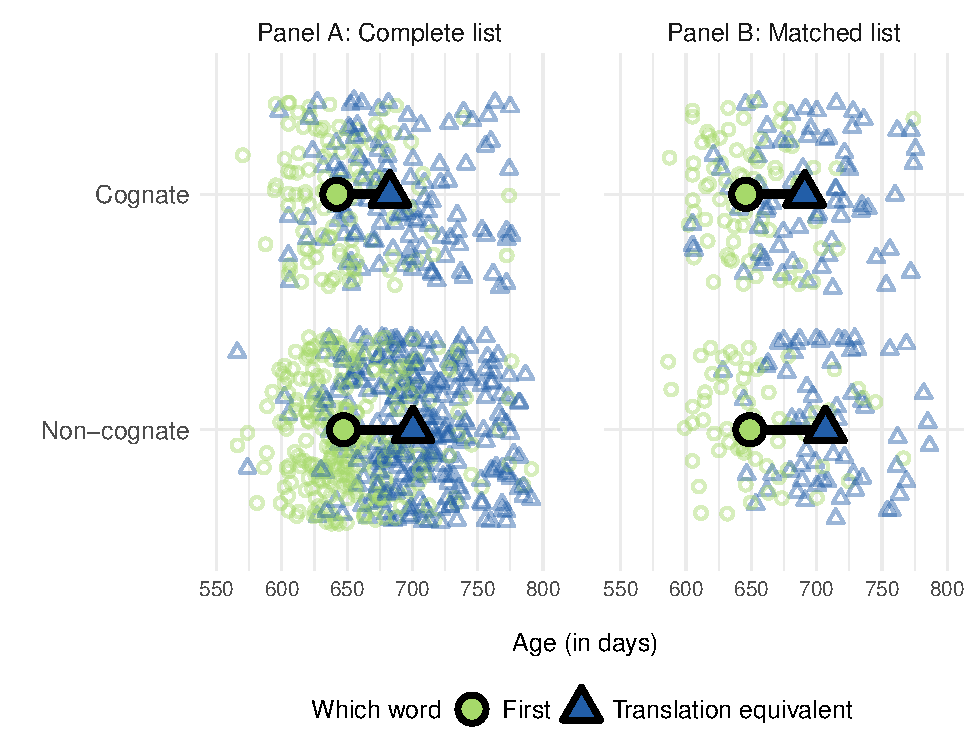
\includegraphics[width=1.2\linewidth]{CogVocab_paper_files/figure-latex/Fig3-1} 

}

\caption{Average intervals between production of the first words (light green circles) and their translation equivalent (dark blue triangles), by cognate status and age. Panel A represents the complete list and Panel B represents the matched list. Smaller individual circles and triangles plot data of the first words and translation equivalent words, respectively, from each word pair.}\label{fig:Fig3}
\end{figure}

\hypertarget{complete-list-2}{%
\subsubsection{Complete List}\label{complete-list-2}}

After having produced a word, on average, bilingual infants took 40.55 days (\(SD\) = 25.81, range = 0 -- 182) to produce its translation equivalent when it was a cognate and 53.19 days (\(SD\) = 30.54, range = 0 -- 221) to produce it when it was a non-cognate. Figure 3 Panel A visualizes this model. The effect of cognate status was statistically significant, \(estimate\) = -9.50, \(SE\) = 2.95, \(t\) = -3.23, \(p\) \textless{} .01. This suggests that once a word was produced, it took bilingual infants a shorter period of time to produce its translation equivalent if it was a cognate than if it was a non-cognate.

\hypertarget{matched-list-2}{%
\subsubsection{Matched List}\label{matched-list-2}}

After having produced a word, on average, bilingual infants took 45.13 days (\(SD\) = 26.20, range = 0 -- 182) to produce its translation equivalent when it was a cognate and 57.89 days (\(SD\) = 31.95, range = 0 -- 221) to produce it when it was a non-cognate. Figure 3 Panel B visualizes this model. Similar to the model for the complete list, we also observed a significant effect of cognate status, \(estimate\) = -12.59, \(SE\) = 4.42, \(t\) = -2.85, \(p\) \textless{} .01. Overall, once infants produced a word, they produced its translation equivalent earlier when the words were cognates than when they were non-cognates.

\hypertarget{summary-of-analyses}{%
\subsection{Summary of Analyses}\label{summary-of-analyses}}

Overall, the result patterns were largely consistent across our analyses. First, bilingual infants produced a greater proportion of cognates than non-cognates. Infants increased their production of both cognates and non-cognates across age, and for the complete list (although not the matched list) this increase was slightly steeper for non-cognates than cognates, although production of cognates remained proportionally greater than that of cognates at the oldest age we observed (27 months). Second, looking at the interval between learning to produce a first and a second word in a translation equivalent pair, this was shorter for cognate than for non-cognate translation equivalents. However, we note that the magnitude of this effect is fairly small, with both cognates and non-cognates first produced on average 1.5--2 months after its translation equivalent was first produced.

\hypertarget{discussion}{%
\section{Discussion}\label{discussion}}

This current study evaluated whether phonological similarity facilitates vocabulary learning in bilinguals, by examining whether cognates are advantaged in bilingual infants' early vocabulary production. Using monthly expressive vocabulary data, our longitudinal dataset revealed an overall advantage for cognates in infancy. Across ages, infants produced proportionally more cognates (e.g., English ``banana'' \textipa{/b@n\ae{}n@/}--French \emph{''banane''} \textipa{/b\textscripta{}n\textscripta{}n/}) than non-cognates (e.g., English ``apple'' \textipa{/\ae{}p@l/}--French \emph{''pomme''} \textipa{/p\textopeno{}m/}), although note that in raw terms children still produced a greater number of non-cognates than cognates, due to the greater absolute frequency of non-cognate translation equivalents on the French--English CDI checklists. Moreover, having produced a word, on average it took infants a shorter period of time (approximately 10--15 days less) to start producing its translation equivalent if the words were cognates than if they were non-cognates.

Together with previous findings, our results begin to paint a developmental picture of the effects of cognate status on early vocabulary productions. Spanish and Catalan have both form-similar and form-identical cognates, and Bosch \& Ramon-Casas (2014) reported a cognate advantage for form-identical but not form-similar cognates at 18 months. Cognates in French and English are almost exclusively form-similar, and we found an advantage for these form-similar in infants aged 16 to 27 months. Other studies have also reported an advantage for non-cognate translation equivalents (Bilson et al., 2015), which might vary with age (Tsui et al., 2022). Overall, translation equivalents with the largest phonological overlap appear to be the most advantaged in early production and thus their effect might be detectable from age 18 months, with potential advantages in children's production of form-similar and non-cognate translation equivalents strengthening across the second and third year of life.

The robust cognate advantage across different bilingual infant populations points to the possibility that the origin of the cognate facilitation effect observed in childhood and in adulthood emerges from infancy. Previous studies which examined the cognate facilitation effect in bilingual adults and school-aged children have reported that bilinguals are better at processing cognates; for example, they can identify and/or name cognates more easily and quickly in a vocabulary task (Costa et al., 2000; Kelley \& Kohnert, 2012; Sheng et al., 2016). Thus, the cognate facilitation effect appears to be robust in vocabulary production across the lifespan, with the advantage for cognates in production emerging early on, as our study results suggested.

We interpret these results in light of theories that emphasize the interconnectedness of the two languages in the developing bilingual lexicon (DeAnda et al., 2016). Studies show that, even across languages, words that are semantically related are acquired sooner by bilingual children (Bilson et al., 2015) and are co-activated in language processing (e.g., DeAnda \& Friend, 2020; Jardak \& Byers-Heinlein, 2018; Singh, 2014). Moreover, young monolinguals find it easier to learn words that are phonologically similar to one another (Coady \& Aslin, 2003; Demke et al., 2002; Jones \& Brandt, 2019), and young bilinguals co-activate phonologically-related words both within and across languages (Von Holzen \& Mani, 2012). These two sets of findings were confirmed in a study of monolingual children across 10 languages, who were more likely to acquire words with a high degree of semantic or phonological association (Fourtassi et al., 2020). Unique to bilinguals, cognates have a high degree of both semantic and phonological overlap, which our results show facilitate their acquisition.

There are several specific ways that cognates' phonological and semantic overlap might advantage their learning. One possibility is that, for cognates, bilingual children might only need to map one phonological form (or slightly varied phonological forms for the cases of form-similar cognates) to label the same referent across the two languages, whereas for non-cognate translation equivalents bilingual children have to memorize two completely different forms for the same referent. Indeed, bilingual children learning similar languages learn more cognate translation equivalents and have a larger vocabulary size in general (Gampe et al., 2021). Thus, transfer effects could explain the cognate advantage we observed in production, and would predict an early-emerging cognate advantage for word comprehension as well. Another possibility is that hearing a cognate word activates and strengthens phonological representations for both languages (e.g., hearing ``banana'' could activate and strengthen both ``banana'' and \emph{``banane''}), thus accelerating cognate learning (Schott et al., 2022). Bilingual children have been found to identify and name cognates easier and faster than non-cognates, suggesting that the phonological overlap in cognates could support bilinguals' lexical decoding and processing (Kelley \& Kohnert, 2012; Sheng et al., 2016). Finally, the closer the phonological form of cognates, the more similar they might be for children to articulate. Support for such a hypothesis comes from study which showed that bilingual children not only learned phonologically-similar words faster but produced phonologically-similar nouns more frequently and more evenly than form-dissimilar nouns across their two languages (Schelletter, 2002). Note that these three possible mechanisms are not mutually exclusive, and could each contribute to the cognate advantage we observed.

There are several other factors that could also contribute to children's faster learning of cognates than non-cognates. For example, Bosch \& Ramon-Casas (2014) brought up several additional possibilities including frequency in the language input, reference to more complex concepts, or production difficulty due to changes in phonological forms, although they could not provide direct evidence due to the limited items on their vocabulary checklists. Our study attempted to account for several of these factors, by analyzing a subset of cognates and non-cognates that were carefully matched for part of speech, typical age of acquisition, and word category when possible. With this carefully controlled subset, we again found a production advantage for cognates. Thus, while such additional factors could potentially contribute to the cognate advantage, our results suggest that such third variable explanations are unlikely to underlie our results.

The cognate advantage can, at least in part, explain why bilingual children learning more similar languages show accelerated vocabulary development relative to bilinguals acquiring less similar languages (Blom et al., 2020; Gampe et al., 2021; Sheng et al., 2016). It has been shown that the more overlap shared across the two languages, the easier the words are learned by bilingual children (Bosma et al., 2019). Therefore, for those who are learning close language pairs that share a high degree of phonological overlap like Spanish and Catalan, their two languages share many cognates which sometimes are even form-identical, meaning that they are pronounced the same way in both languages (e.g, \emph{``sí''} /si/ meaning ``yes'' in both languages). On the other hand, for those who are learning languages that share a lesser degree of phonological similarity like English and French, there are potentially very few form-identical cognates. It is possible that when languages are very similar and share many form-identical cognates, bilingual infants can benefit from these words from a very young age. On the other hand, when languages are somewhat less similar and share mostly form-similar cognates, children may need more time to detect and benefit from cognates. Overall, we suggest that there is a gradual timeline for the facilitative effect of cognates in infancy, which starts off with form-identical cognates then form-similar cognates (Bosma et al., 2019). Future studies could include additional language pairs which are less similar than Spanish and Catalan but more similar than English and French, such as Spanish and Italian (Schepens et al., 2013), to directly compare the timeline regarding the acquisition of form-identical cognates, form-similar cognates, and non-cognates. Moreover, while previous studies suggested that bilingual children learning more similar languages learned more translation equivalent pairs than those learning less similar languages (Gampe et al., 2021), it would also be important for future studies to further examine whether the advantage for cognates is of the same nature across different language pairs. A final interesting direction would be to use a continuous metric to quantify the degree of phonological overlap in form-similar cognate pairs, to more precisely examine how phonological overlap contributes to word learning.

An important avenue for future research would be to examine whether the same cognate advantage would be observed in receptive vocabulary acquisition, and indeed some evidence points in this direction. Some work with Spanish-Catalan bilinguals has suggested that infants show less perceptual sensitivity to cross-language phonological distinctions in cognates due to their phonological similarity (Ramon-Casas et al., 2009; Ramon-Casas \& Bosch, 2010), suggesting that cognates may hold a different status in early bilinguals' receptive lexicons compared to non-cognates. However, more recent research with French--English bilingual toddlers had an opposite finding, whereby cognates were represented in more phonetic detail than non-cognates (Schott et al., 2022). There is also evidence that the cognate advantage is modulated by the level of difficulty of the vocabulary item for both comprehension and production. One study found that although the cognate advantage was observed in easier items, the effect was even greater in vocabulary items that were considered to be medium or hard (Kelley \& Kohnert, 2012). This may suggest that infants would have a cognate advantage in any vocabulary task---either receptive or expressive, especially for less-familiar words where they may use the cognate word they have already acquired for help (Kelley \& Kohnert, 2012), which is the case when infants are acquiring new words and learning to pronounce them. Therefore, we could expect a cognate advantage in both comprehension and production, serving different purposes: in comprehension, a cognate advantage would help activate the representations for the words in both languages, whereas in production, cognates may also facilitate the acquisition of the word in the individuals' other language in terms of pronunciation, as was seen in our study. Future research could explore the difference between comprehension and production in bilingual infants' language acquisition while simultaneously looking at the cognate advantage. Moreover, future studies could also consider looking into the advantage for cognates and its impact on bilingual children's online production or pronunciation of cognate words. Finally, we note that our current study made use of the MacArthur CDIs as checklists to assess bilingual infants' vocabulary production. While the use of the vocabulary checklists allowed us to systematically compare bilingual infants' vocabulary across their two languages, it is likely that infants produced translation equivalents that were not on these measures. The use of other methodologies including day-long recording to explore infants' real-life cognate production remains open for future studies.

\hypertarget{conclusion}{%
\section{Conclusion}\label{conclusion}}

The present study demonstrated that French--English bilingual infants show an advantage for cognates in vocabulary production. Infants produced proportionally more cognates than non-cognates, and the interval between producing a word and its translation equivalent was shorter for cognates than non-cognates. These findings can, at least in part, explain why children learning typologically similar languages show faster vocabulary growth than those learning more distant languages (Blom et al., 2020; Gampe et al., 2021; Sheng et al., 2016). Altogether, our study provides a greater understanding of the effect of similar-sounding words on infants' language acquisition over time. Future studies with data from other populations of bilinguals will be important to more fully understand the effect of the cognate advantage in early bilingual vocabulary development.

\newpage

\hypertarget{acknowledgements}{%
\section{Acknowledgements}\label{acknowledgements}}

\noindent The present research was approved by the Human Research Ethics Committee at Concordia University {[}certification \#10000439{]}. We are grateful to all the families who participated in this research. This manuscript derives from a thesis submitted by Lori Mitchell in partial fulfilment for an honours degree in Psychology at Concordia University. This work was supported by grants to Byers-Heinlein from the Natural Sciences and Engineering council of Canada {[}2018-04390{]}) and the National Institutes of Health {[}1R01HD095912-01A1{]}. Byers-Heinlein holds the Concordia University Research Chair in Bilingualism and Open Science. This study has been presented as a poster at the 2021 Boston University Conference on Language Development, and the data has also been presented as a talk at the 2022 International Congress of Infant Studies. We thank the members of the Concordia Infant Research Lab for their comments on earlier versions of this paper.

\newpage

\hypertarget{references}{%
\section{References}\label{references}}

\begingroup
\setlength{\parindent}{-0.5in}

\hypertarget{refs}{}
\begin{CSLReferences}{1}{0}
\leavevmode\vadjust pre{\hypertarget{ref-Bates_etal_2015}{}}%
Bates, M., D., \& Walker, S. (2015). Fitting linear mixed-effects models using lme4. \emph{Journal of Statistical Software}, \emph{67}(1), 1--48. \url{https://doi.org/10.18637/jss.v067.i01}

\leavevmode\vadjust pre{\hypertarget{ref-Bilson_etal_2015}{}}%
Bilson, S., Yoshida, H., Tran, C. D., Woods, E. A., \& Hills, T. T. (2015). Semantic facilitation in bilingual first language acquisition. \emph{Cognition}, \emph{140}, 122--134. \url{https://doi.org/10.1016/j.cognition.2015.03.013}

\leavevmode\vadjust pre{\hypertarget{ref-Blom_etal_2019}{}}%
Blom, B., E., \& Timmermeister, M. (2019). Cross-language distance influences receptive vocabulary outcomes of bilingual children. \emph{First Language}, \emph{40}(2), 151--171. \url{https://doi.org/10.1177/0142723719892794}

\leavevmode\vadjust pre{\hypertarget{ref-Bosch_Ramon-Casas_2014}{}}%
Bosch, L., \& Ramon-Casas, M. (2014). First translation equivalents in bilingual toddlers' expressive vocabulary: Does form similarity matter? \emph{International Journal of Behavioral Development}, \emph{38}(4), 317--322. \url{https://doi.org/10.1177/0165025414532559}

\leavevmode\vadjust pre{\hypertarget{ref-Bosch_Sebastian-Galles_2001}{}}%
Bosch, L., \& Sebastián-Gallés, N. (2001). Evidence of early language discrimination abilities in infants from bilingual environments. \emph{Infancy}, \emph{21}(1), 29--49. \url{https://doi.org/10.1207/S15327078IN0201_3}

\leavevmode\vadjust pre{\hypertarget{ref-Bosma_etal_2019}{}}%
Bosma, E., Blom, E., Hoekstra, E., \& Versloot, A. (2019). A longitudinal study on the gradual cognate facilitation effect in bilingual children's {F}risian receptive vocabulary. \emph{International Journal of Bilingual Education and Bilingualism}, \emph{22}(4), 371--385. \url{https://doi.org/doi.org/10.1080/13670050.2016.1254152}

\leavevmode\vadjust pre{\hypertarget{ref-Byers-Heinlein_etal_2023}{}}%
Byers-Heinlein, K., Gonzalez-Barrero, A. M., Schott, E., \& Killam, H. (in press, 2023). Sometimes larger, sometimes smaller: Measuring vocabulary in monolingual and bilingual infants and toddlers. \emph{First Language}. \url{https://doi.org/10.31234/osf.io/x7s4u}

\leavevmode\vadjust pre{\hypertarget{ref-Byers-Heinlein_etal_2020}{}}%
Byers-Heinlein, K., Schott, E., Gonzalez-Barrero, A. M., Brouillard, M., Dubé, D., Jardak, A., \ldots{} Tamayo, M. P. (2020). MAPLE: A multilingual approach to parent language estimates. \emph{Bilingualism: Language and Cognition}, \emph{23}(5), 951--957. \url{https://doi.org/10.1017/S1366728919000282}

\leavevmode\vadjust pre{\hypertarget{ref-Caselli_etal_1995}{}}%
Caselli, B., M. C., \& Weir, J. (1995). A cross-linguistic study of early lexical development. \emph{Cognitive Development}, \emph{10}(2), 159--199. \url{https://doi.org/10.1016/0885-2014(95)90008-x}

\leavevmode\vadjust pre{\hypertarget{ref-Choi_2019}{}}%
Choi, H. (2019). Strategy training for {E}nglish-{F}rench cognate awareness: Contributions to {K}orean learners' L3 {F}rench competency. \emph{Electronic Journal of Foreign Language Teaching}, \emph{16}(1), 68--79. Retrieved from \url{https://e-flt.nus.edu.sg/wp-content/uploads/2020/09/choi.pdf}

\leavevmode\vadjust pre{\hypertarget{ref-Cnaan_etal_1997}{}}%
Cnaan, A., Laird, N. M., \& Slasor, P. (1997). Using the general linear mixed model to analyse unbalanced repeated measures and longitudinal data. \emph{Statistics in Medicine}, \emph{16}(20), 2349--2380. \url{https://doi.org/10.1002/(SICI)1097-0258(19971030)16:20\%3C2349::AID-SIM667\%3E3.0.CO;2-E}

\leavevmode\vadjust pre{\hypertarget{ref-Cody_Aslin_2003}{}}%
Coady, J. A., \& Aslin, R. N. (2003). Phonological neighbourhoods in the developing lexicon. \emph{Journal of Child Language}, \emph{30}(2), 441--469. \url{https://doi.org/10.1017/S0305000903005579}

\leavevmode\vadjust pre{\hypertarget{ref-Costa_etal_2000}{}}%
Costa, C., A., \& Sebastian-Galles, N. (2000). The cognate facilitation effect: Implications for models of lexical access. \emph{Journal of Experimental Psychology: Learning, Memory, and Cognition}, \emph{26}(5), 1283--1296. \url{https://doi.org/10.1037/0278-7393.26.5.1283}

\leavevmode\vadjust pre{\hypertarget{ref-DeHouwer_etal_2006}{}}%
De Houwer, A., Bornstein, M. H., \& De Coster, S. (2006). Early understanding of two words for the same thing: A {CDI} study of lexical comprehension in infant bilinguals. \emph{International Journal of Bilingualism}, \emph{10}(3), 331--347. \url{https://doi.org/10.1177/13670069060100030401}

\leavevmode\vadjust pre{\hypertarget{ref-DeAnda_Friend_2020}{}}%
DeAnda, S., \& Friend, M. (2020). Lexical-semantic development in bilingual toddlers at 18 and 24 months. \emph{Frontiers in Psychology}, \emph{11}, 3500. \url{https://doi.org/10.3389/fpsyg.2020.508363}

\leavevmode\vadjust pre{\hypertarget{ref-DeAnda_etal_2016}{}}%
DeAnda, S., Poulin-Dubois, D., Zesiger, P., \& Friend, M. (2016). Lexical processing and organization in bilingual first language acquisition: Guiding future research. \emph{Psychological Bulletin}, \emph{142}(6), 655--667. \url{https://doi.org/10.1037/bul0000042}

\leavevmode\vadjust pre{\hypertarget{ref-Demke_etal_2002}{}}%
Demke, G., T. L., \& Siakaluk, P. D. (2002). The influence of exposure to phonological neighbours on preschoolers' novel word production. \emph{Journal of Child Language}, \emph{29}(2), 379--392. \url{https://doi.org/10.1017/S0305000902005081}

\leavevmode\vadjust pre{\hypertarget{ref-Fenson_etal_2007}{}}%
Fenson, L., Marchman, V. A., Thal, D. J., Dale, P. S., Reznick, J. S., \& Bates, E. (2007). \emph{MacArthur-{B}ates {C}ommunicative {D}evelopment {I}nventories ({CDIs})} (2nd ed.). Baltimore, MD: Brookes Publishing.

\leavevmode\vadjust pre{\hypertarget{ref-Floccia_etal_2020}{}}%
Floccia, C., Luche, C. D., Lepadatu, I., Chow, J., Ratnage, P., \& Plunkett, K. (2020). Translation equivalent and cross-language semantic priming in bilingual toddlers. \emph{Journal of Memory and Language}, \emph{112}, 104086. \url{https://doi.org/10.1016/j.jml.2019.104086}

\leavevmode\vadjust pre{\hypertarget{ref-Fourtassi_etal_2020}{}}%
Fourtassi, A., Bian, Y., \& Frank, M. C. (2020). The growth of children's semantic and phonological networks: Insight from 10 languages. \emph{Cognitive Science}, \emph{44}(7), e12847. \url{https://doi.org/10.1111/cogs.12847}

\leavevmode\vadjust pre{\hypertarget{ref-Frank_etal_2017}{}}%
Frank, M. C., Braginsky, M., Yurovsky, D., \& Marchman, V. A. (2017). Wordbank: An open repository for developmental vocabulary data. \emph{Journal of Child Language}, \emph{44}(3), 677--694. \url{https://doi.org/10.1017/S0305000916000209}

\leavevmode\vadjust pre{\hypertarget{ref-Gampe_etal_2021}{}}%
Gampe, Q., A., \& Daum, M. M. (2021). Does linguistic similarity affect early simultaneous bilingual language acquisition? \emph{Journal of Language Contact}, \emph{13}(3), 482--500. \url{https://doi.org/10.1163/19552629-13030001}

\leavevmode\vadjust pre{\hypertarget{ref-Hanson_Klopfer_2006}{}}%
Hansen, B. B., \& Klopfer, S. O. (2006). Optimal full matching and related designs via network flows. \emph{Journal of Computational and Graphical Statistics}, \emph{15}(3), 609--627. \url{https://doi.org/10.1198/106186006X137047}

\leavevmode\vadjust pre{\hypertarget{ref-Hartig_2022}{}}%
Hartig, F. (2022). \emph{DHARMa: Residual diagnostics for hierarchical (multi-level/mixed) regression models}. R package version 0.4.5. Retrieved from \url{https://CRAN.R-project.org/package=DHARMa}

\leavevmode\vadjust pre{\hypertarget{ref-Havy_etal_2016}{}}%
Havy, B., M., \& Nazzi, T. (2016). Phonetic processing when learning words: The case of bilingual infants. \emph{International Journal of Behavioral Development}, \emph{40}(1), 41--52. \url{https://doi.org/10.1177/0165025415570646}

\leavevmode\vadjust pre{\hypertarget{ref-Hoff_Ribot_2017}{}}%
Hoff, E., \& Ribot, K. M. (2017). Language growth in {E}nglish monolingual and {S}panish-{E}nglish bilingual children from 2.5 to 5 years. \emph{The Journal of Pediatrics}, \emph{190}, 241--245. \url{https://doi.org/10.1016/j.jpeds.2017.06.071}

\leavevmode\vadjust pre{\hypertarget{ref-Jardak_Byers-Heinlein_2019}{}}%
Jardak, A., \& Byers-Heinlein, K. (2019). Labels or concepts? The development of semantic networks in bilingual two-year-olds. \emph{Child Development}, \emph{90}(2), e212--e229. \url{https://doi.org/10.1111/cdev.13050}

\leavevmode\vadjust pre{\hypertarget{ref-Jones_Brandt_2019}{}}%
Jones, S., \& Brandt, S. (2019). Do children really acquire dense neighbourhoods? \emph{Journal of Child Language}, \emph{46}(6), 1260--1273. \url{https://doi.org/10.1017/S0305000919000473}

\leavevmode\vadjust pre{\hypertarget{ref-Kelley_Kohnert_2012}{}}%
Kelley, A., \& Kohnert, K. (2012). Is there a cognate advantage for typically developing {S}panish-speaking {E}nglish-language learners? \emph{Language, Speech, and Hearing Services in Schools}, \emph{43}(2), 191--204. \url{https://doi.org/10.1044/0161-1461(2011/10-0022)}

\leavevmode\vadjust pre{\hypertarget{ref-Kuznetsova_etal_2017}{}}%
Kuznetsova A., P. B., Brockhoff, \& Christensen, R. H. B. (2017). lmerTest package: Tests in linear mixed effects models. \emph{Journal of Statistical Software}, \emph{82}(13), 1--26. \url{https://doi.org/10.18637/jss.v082.i13}

\leavevmode\vadjust pre{\hypertarget{ref-Legacy_etal_2017}{}}%
Legacy, J., Reider, J., Crivello, C., Kuzyk, O., Friend, M., Zesiger, P., \& Poulin-Dubois, D. (2017). Dog or chien? Translation equivalents in the receptive and expressive vocabularies of young {F}rench--{E}nglish bilinguals. \emph{Journal of Child Language}, \emph{44}(4), 881--904. \url{https://doi.org/10.1017/S0305000916000295}

\leavevmode\vadjust pre{\hypertarget{ref-Luce_Pisoni_1998}{}}%
Luce, P. A., \& Pisoni, D. B. (1998). Recognizing spoken words: The neighborhood activation model. \emph{Ear and Hearing}, \emph{19}, 1. \url{https://doi.org/10.1097/00003446-199802000-00001}

\leavevmode\vadjust pre{\hypertarget{ref-Marchman_etal_2010}{}}%
Marchman, V. A., Fernald, A., \& Hurtado, N. (2010). How vocabulary size in two languages relates to efficiency in spoken word recognition by young {S}panish-{E}nglish bilinguals. \emph{Journal of Child Language}, \emph{37}(4), 817--840. \url{https://doi.org/10.1017/S0305000909990055}

\leavevmode\vadjust pre{\hypertarget{ref-Morin-Lessard_Byers-Heinlein_2019}{}}%
Morin-Lessard, E., \& Byers-Heinlein, K. (2019). Uh and euh signal novelty for monolinguals and bilinguals: Evidence from children and adults. \emph{Journal of Child Language}, \emph{46}(3), 522--545. \url{https://doi.org/10.1017/s0305000918000612}

\leavevmode\vadjust pre{\hypertarget{ref-Pearson_etal_1995}{}}%
Pearson, B. Z., Fernández, S. C., \& Oller, D. K. and. (1995). Cross-language synonyms in the lexicons of bilingual infants: One language or two? \emph{Journal of Child Language}, \emph{22}(2), 345--368. \url{https://doi.org/10.1017/s030500090000982x}

\leavevmode\vadjust pre{\hypertarget{ref-Place_Hoff_2011}{}}%
Place, S., \& Hoff, E. (2011). Properties of dual language exposure that influence 2-year-olds' bilingual proficiency. \emph{Child Development}, \emph{82}(6), 1834--1849. \url{https://doi.org/10.1111/j.1467-8624.2011.01660.x}

\leavevmode\vadjust pre{\hypertarget{ref-R_2019}{}}%
R Core Team. (2019). \emph{R: A language and environment for statistical computing}. Vienna, Austria: R Foundation for Statistical Computing. Retrieved from \url{https://www.R-project.org/}

\leavevmode\vadjust pre{\hypertarget{ref-Ramon-Casas_Bosch_2010}{}}%
Ramon-Casas, M., \& Bosch, L. (2010). Are non-cognate words phonologically better specified than cognates in the early lexicon of bilingual children? In \emph{Proceedings of the 4th conference on laboratory approaches to spanish phonology} (pp. 31--36). Sommerville, MA: Cascadilla.

\leavevmode\vadjust pre{\hypertarget{ref-Ramon-Casas_etal_2009}{}}%
Ramon-Casas, S., M., \& Bosch, L. (2009). Vowel categorization during word recognition in bilingual toddlers. \emph{Cognitive Psychology}, \emph{59}(1), 96--121. \url{https://doi.org/10.1016/j.cogpsych.2009.02.002}

\leavevmode\vadjust pre{\hypertarget{ref-Rocha_Barr_2022}{}}%
Rocha-Hidalgo, J., \& Barr, R. (2022). Defining bilingualism in infancy and toddlerhood: A scoping review. \emph{International Journal of Bilingualism}, \emph{0}(0). \url{https://doi.org/10.1177/13670069211069067}

\leavevmode\vadjust pre{\hypertarget{ref-Schelletter_2002}{}}%
Schelletter, C. (2002). The effect of form similarity on bilingual children's lexical development. \emph{Bilingualism: Language and Cognition}, \emph{5}(2), 93--107. \url{https://doi.org/10.1017/S1366728902000214}

\leavevmode\vadjust pre{\hypertarget{ref-Schepens_etal_2013}{}}%
Schepens, J., Dijkstra, T., Grootjen, F., \& Heuven, W. J. B. van. (2013). Cross-language distributions of high frequency and phonetically similar cognates. \emph{PLOS ONE}, \emph{8}(5), e63006. \url{https://doi.org/10.1371/journal.pone.0063006}

\leavevmode\vadjust pre{\hypertarget{ref-Schott_etal_2022}{}}%
Schott, E., Moore, C., \& Byers-Heinlein, K. (2022). \emph{Banana and banane: Cross-language phonological overlap supports bilingual toddlers' word representations}. Preprint. \url{https://doi.org/10.31219/osf.io/hgdvq}

\leavevmode\vadjust pre{\hypertarget{ref-Sebastiuxe1n-Galluxe9s_Bosch_2009}{}}%
Sebastián-Gallés, N., \& Bosch, L. (2009). Developmental shift in the discrimination of vowel contrasts in bilingual infants: Is the distributional account all there is to it? \emph{Developmental Science}, \emph{12}(6), 874--887. \url{https://doi.org/10.1111/j.1467-7687.2009.00829.x}

\leavevmode\vadjust pre{\hypertarget{ref-Sheng_etal_2016}{}}%
Sheng, L., L., \& Fulton, A. (2016). A robust demonstration of the cognate facilitation effect in first-language and second-language naming. \emph{Journal of Experimental Child Psychology}, \emph{141}, 229--238. \url{https://doi.org/10.1016/j.jecp.2015.09.007}

\leavevmode\vadjust pre{\hypertarget{ref-Singh_2014}{}}%
Singh, L. (2014). One world, two languages: Cross-language semantic priming in bilingual toddlers. \emph{Child Development}, \emph{85}(2), 755--766. \url{https://doi.org/10.1111/cdev.12133}

\leavevmode\vadjust pre{\hypertarget{ref-Storkel_2009}{}}%
Storkel, H. L. (2009). Developmental differences in the effects of phonological, lexical and semantic variables on word learning by infants. \emph{Journal of Child Language}, \emph{36}(2), 291--321. \url{https://doi.org/10.1017/S030500090800891X}

\leavevmode\vadjust pre{\hypertarget{ref-Trudeau_etal_1999}{}}%
Trudeau, N., Frank, I., \& Poulin-Dubois, D. (1999). Une adaptation en français québecois du MacArthur {C}ommunicative {D}evelopment {I}nventory {[}a {Q}uebec {F}rench adaptation of the MacArthur {C}ommunicative {D}evelopment {I}nventory{]}. \emph{Revue d'orthophonie Et d'audiologie}, \emph{23}, 31--73.

\leavevmode\vadjust pre{\hypertarget{ref-Tsui_etal_2022}{}}%
Tsui, R. K.-Y., Gonzalez-Barrero, A. M., Schott, E., \& Byers-Heinlein, K. (2022). Are translation equivalents special? Evidence from simulations and empirical data from bilingual infants. \emph{Cognition}, \emph{225}, 105084. \url{https://doi.org/10.1016/j.cognition.2022.105084}

\leavevmode\vadjust pre{\hypertarget{ref-Volterra_Taeschner_1978}{}}%
Volterra, V., \& Taeschner, T. (1978). The acquisition and development of language by bilingual children. \emph{Journal of Child Language}, \emph{5}, 311--326. \url{https://doi.org/10.1017/S0305000900007492}

\leavevmode\vadjust pre{\hypertarget{ref-VonHolzen_Mani_2012}{}}%
Von Holzen, K., \& Mani, N. (2012). Language nonselective lexical access in bilingual toddlers. \emph{Journal of Experimental Child Psychology}, \emph{113}(4), 569--586. \url{https://doi.org/10.1016/j.jecp.2012.08.001}

\leavevmode\vadjust pre{\hypertarget{ref-White_etal_2017}{}}%
White, M., A., \& Storms, G. (2017). Convergence in the bilingual lexicon: A pre-registered replication of previous studies. \emph{Frontiers in Psychology}, \emph{7}, 2081. \url{https://doi.org/10.3389/fpsyg.2016.02081}

\end{CSLReferences}

\endgroup


\end{document}
